\documentclass[11pt]{article}
\usepackage{ctex}
\usepackage[english]{babel}
\usepackage{blindtext}
\usepackage{nameref}
\usepackage{fancyhdr}
\usepackage{tabularx}
\usepackage{amsmath,amssymb,amsthm}
\usepackage{graphicx,float}
\usepackage{physics}
\usepackage{pgfplots}
\usepackage[a4paper, total={6in, 9in}]{geometry}
\usepackage{wrapfig}

\graphicspath{{../images/}}

\pagestyle{fancy}
\fancyhf{}
\fancyhf[HL]{F4 Final practice paper}
\fancyhf[CF]{\thepage}

\newcommand{\innerprod}[2]{\langle{#1},{#2}\rangle}
\newcommand{\id}{\mathtt{id}}

\newtheorem*{definition}{Definition}
\newtheorem*{theorem}{Theorem}
\newtheorem*{corollary}{Corollary}
\newtheorem*{lemma}{Lemma}
\newtheorem*{proposition}{Proposition}
\newtheorem*{remark}{Remark}
\newtheorem*{claim}{Claim}
\newtheorem*{example}{Example}
\newtheorem*{axiom}{Axiom}

\begin{document}
    \thispagestyle{plain}

    \centering 

    \section*{PRACTICE QUESTIONS\\MATHEMATICS Compulsory Part\\Question-Answer Book}

    \raggedright

    \subsection*{Instructions}

    \begin{enumerate}
        \item This paper must be answered in English.
        \item Unless otherwise specified, all working must be clearly shown.
        \item Unless otherwise specified, numerical answers must be exact.
        \item This paper is for \textbf{internal use} only.
        \item All questions are collected from AL/CE/DSE past papers, reference site: https://www.dse.life/ppindex/m2/
    \end{enumerate}

    \newpage

    \begin{enumerate}
        \item Let $f(x)=\dfrac{1}{2}x-\dfrac{1}{144}x^2-6$. Using the method of completing the sqaure, find the coordinates of the vertex of the graph of $y=f(x)$.
        
            \hrulefill
                
            \hrulefill
            
            \hrulefill
        
            \hrulefill
            
            \hrulefill
                
            \hrulefill
            
            \hrulefill
                
            \hrulefill
            
            \hrulefill
            
            \hrulefill
            
            \hrulefill
            
            \hrulefill
            
            \hrulefill
            
            \hrulefill
            
            \hrulefill
            
            \hrulefill
            
            \hrulefill
            
            \hrulefill
            
            \hrulefill
            
            \hrulefill
            
            \hrulefill
            
            \hrulefill
            
            \hrulefill
            
            \hrulefill
            
            \hrulefill
            
            \hrulefill
            
            \hrulefill
            
            \hrulefill
            
            \hrulefill

        \pagebreak
        \item Let $C(k)$ be the curve $y=\dfrac{1}{k+1}[2x^2+(k+7)x+4]$, where $k\neq -1$.\begin{enumerate}
            \item If $C(k)$ cuts the x-axis at two points at $P$ and $Q$, and $PQ=1$, find the value(s) of $k$.
            \item Find the range of values of $k$ such that $C(k)$ does not cut the x-axis.
            \item \begin{enumerate}
                \item Find the points of intersection of the curves $C(1)$ and $C(2)$.
                \item Show that $C(k)$ passes through the two points in (c)(i) fro all values of $k$. 
            \end{enumerate} 
        \end{enumerate}
        
            \hrulefill
                
            \hrulefill
            
            \hrulefill
            
            \hrulefill
            
            \hrulefill
            
            \hrulefill
            
            \hrulefill
            
            \hrulefill
            
            \hrulefill
            
            \hrulefill
            
            \hrulefill
            
            \hrulefill
            
            \hrulefill
            
            \hrulefill
            
            \hrulefill
            
            \hrulefill
            
            \hrulefill
            
            \hrulefill
            
            \hrulefill
            
            \hrulefill
            
            \hrulefill
            
            \hrulefill
            
            \hrulefill

        \pagebreak
        \item \begin{enumerate}
            \item Let $f(x)=36x-x^2$. Using the method of completing the sqaure, find the coordinates of the vertex of the graph of $y=f(x)$.
            \item The length of a piece of string is 108m. A guard cuts the string into two pieces. One piece is used to enclose a rectangular restricted zone of area $A$ m$^2$. The other piece is used to divide this restricted zone into two rectangular regions as shown in the figure.\begin{figure}[H]
                \centering
                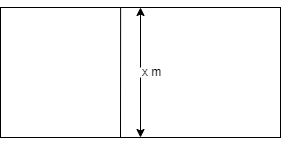
\includegraphics[scale=0.4]{f4finalq3.png}
            \end{figure}\begin{enumerate}
                \item Express $A$ in terms of $x$.
                \item The guard claims that the area of this restricted zone can be greater than 500 m$^{2}$. Do you agree? Explain your answer.
            \end{enumerate}
        \end{enumerate}
        
            \hrulefill
                
            \hrulefill

            \hrulefill
            
            \hrulefill
        
            \hrulefill
            
            \hrulefill
                
            \hrulefill
            
            \hrulefill
                
            \hrulefill
            
            \hrulefill
            
            \hrulefill
            
            \hrulefill
            
            \hrulefill

            \hrulefill
            
            \hrulefill
        
            \hrulefill
            
            \hrulefill
                
            \hrulefill
            
            \hrulefill
            
            \hrulefill
            
            \hrulefill
            
            \hrulefill
        
            \hrulefill
            
            \hrulefill
                
            \hrulefill
            
            \hrulefill
                
            \hrulefill
            
            \hrulefill
            
            \hrulefill
            
            \hrulefill
            
            \hrulefill
            
            \hrulefill
            
            \hrulefill
            
            \hrulefill
            
            \hrulefill
            
            \hrulefill
            
            \hrulefill
            
            \hrulefill
            
            \hrulefill
            
            \hrulefill
            
            \hrulefill
            
            \hrulefill
            
            \hrulefill
            
            \hrulefill
            
            \hrulefill
            
            \hrulefill
            
            \hrulefill
            
            \hrulefill

        \pagebreak
        \item In the figure, $ABCD$ is a rhombus. The diagonals $AC$ and $BD$ cuts at $E$.\begin{figure}[H]
            \centering
            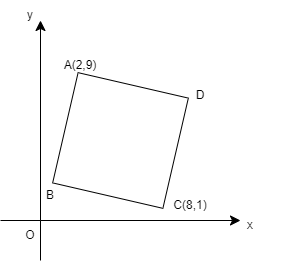
\includegraphics[scale=0.6]{f4finalq4.png}
        \end{figure}\begin{enumerate}
            \item Find\begin{enumerate}
                \item the coordinates of $E$,
                \item the equation of $BD$.
            \end{enumerate}
            \item It is given that the equation of $AD$ is $x+7y-65=0$. Find\begin{enumerate}
                \item the equation of $BC$,
                \item the length of $AB$.
            \end{enumerate}
        \end{enumerate}

            \hrulefill
                    
            \hrulefill

            \hrulefill
            
            \hrulefill
        
            \hrulefill
            
            \hrulefill
                
            \hrulefill
            
            \hrulefill
                
            \hrulefill
            
            \hrulefill
            
            \hrulefill
            
            \hrulefill
            
            \hrulefill

            \hrulefill
            
            \hrulefill
        
            \hrulefill
            
            \hrulefill
                
            \hrulefill
            
            \hrulefill
            
            \hrulefill
            
            \hrulefill
            
            \hrulefill
        
            \hrulefill
            
            \hrulefill
                
            \hrulefill
            
            \hrulefill
                
            \hrulefill
            
            \hrulefill
            
            \hrulefill
            
            \hrulefill
            
            \hrulefill
            
            \hrulefill
            
            \hrulefill
            
            \hrulefill
            
            \hrulefill
            
            \hrulefill
            
            \hrulefill
            
            \hrulefill
            
            \hrulefill
            
            \hrulefill
            
            \hrulefill
            
            \hrulefill
            
            \hrulefill
            
            \hrulefill
            
            \hrulefill

        \pagebreak
        \item In the figure, the straight line passing through $A$ and $B$ is perpendicular to the straight line passing through $A$ and $C$, where $C$ is a point lying on the x-axis.\begin{figure}[H]
            \centering
            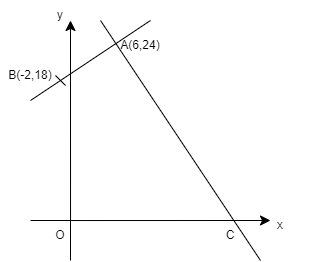
\includegraphics[scale=0.6]{f4finalq5.png}
        \end{figure}\begin{enumerate}
            \item Find the equation of the straigh line passing through $A$ and $B$.
            \item Find the coordinates of $C$.
            \item Find the area of $\triangle ABC$.
            \item A straight line passing through $A$ and the line segment $BC$ at $D$ such that the area of $\triangle ABD$ is 90 square units. Let $BD:DC=r:1$. Find the value of $r$.
        \end{enumerate}
        \hrulefill
                    
            \hrulefill

            \hrulefill
            
            \hrulefill
        
            \hrulefill
            
            \hrulefill
                
            \hrulefill
            
            \hrulefill
                
            \hrulefill
            
            \hrulefill
            
            \hrulefill
            
            \hrulefill
            
            \hrulefill

            \hrulefill
            
            \hrulefill
        
            \hrulefill
            
            \hrulefill
                
            \hrulefill
            
            \hrulefill
            
            \hrulefill
            
            \hrulefill
            
            \hrulefill
        
            \hrulefill
            
            \hrulefill
                
            \hrulefill
            
            \hrulefill
                
            \hrulefill
            
            \hrulefill
            
            \hrulefill
            
            \hrulefill
            
            \hrulefill
            
            \hrulefill
            
            \hrulefill
            
            \hrulefill
            
            \hrulefill
            
            \hrulefill
            
            \hrulefill
            
            \hrulefill
            
            \hrulefill
            
            \hrulefill
            
            \hrulefill
            
            \hrulefill
            
            \hrulefill
            
            \hrulefill
            
            \hrulefill

        \pagebreak
        \item \begin{enumerate}
            \item Factorize $a^4-16$ and $a^3-8$.
            \item Find the L.C.M. of $a^4-16$ and $a^3-8$.
        \end{enumerate}
        \hrulefill
            
            \hrulefill
            
            \hrulefill
            
            \hrulefill
            
            \hrulefill
            
            \hrulefill
            
            \hrulefill
            
            \hrulefill
            
            \hrulefill
            
            \hrulefill
            
            \hrulefill
            
            \hrulefill
            
            \hrulefill
            
            \hrulefill
            
        \item Factorize\begin{enumerate}
            \item $m^2+12mn+36n^2$.
            \item $m^2+12mn+36n^2-s^2$.
        \end{enumerate}
        \hrulefill
            
            \hrulefill
            
            \hrulefill
            
            \hrulefill
            
            \hrulefill
            
            \hrulefill
            
            \hrulefill
            
            \hrulefill
            
            \hrulefill
            
            \hrulefill
            
            \hrulefill

        \pagebreak
        \item Factorize\begin{enumerate}
            \item $x^3+x^2y-7x^2$.
            \item $x^3+x^2y-7x^2-x-y+7$.
        \end{enumerate}
        \hrulefill
            
            \hrulefill
            
            \hrulefill
            
            \hrulefill
            
            \hrulefill
            
            \hrulefill
            
            \hrulefill
            
            \hrulefill
            
            \hrulefill
            
            \hrulefill
            
            \hrulefill

        \item Factorize\begin{enumerate}
            \item $4m^2-9$.
            \item $2m^2n+7mn-15n$.
            \item $4m^2-9-2m^2n-7mn+15n$
        \end{enumerate}
        \hrulefill
            
            \hrulefill
            
            \hrulefill
            
            \hrulefill
            
            \hrulefill
            
            \hrulefill
            
            \hrulefill
            
            \hrulefill
            
            \hrulefill
            
            \hrulefill
            
            \hrulefill

        \pagebreak
        \item It is given that $f(x)=2x^2+ax+b$.\begin{enumerate}
            \item If $f(x)$ is divided by $(x-1)$, the remainder is $-5$. If $f(x)$ is divided by $(x+2)$, the remainder is 4. Find the values of $a$ and $b$.
            \item If $f(x)=0$, find the values of $x$.
        \end{enumerate}
        \hrulefill
            
            \hrulefill
            
            \hrulefill
            
            \hrulefill
            
            \hrulefill
            
            \hrulefill
            
            \hrulefill
            
            \hrulefill
            
            \hrulefill
            
            \hrulefill
            
            \hrulefill

            \hrulefill
            
            \hrulefill
            
            \hrulefill
            
            \hrulefill

            \hrulefill
            
            \hrulefill
            
            \hrulefill
            
            \hrulefill
            
            \hrulefill
            
            \hrulefill
            
            \hrulefill
            
            \hrulefill
            
            \hrulefill
            
            \hrulefill

        \pagebreak
        \item If $3x^2-kx-2$ is divisible by $x-k$, find the two values of $k$.
            
            \hrulefill
                
            \hrulefill
            
            \hrulefill
            
            \hrulefill
            
            \hrulefill
            
            \hrulefill
            
            \hrulefill
            
            \hrulefill
            
            \hrulefill
            
            \hrulefill
            
            \hrulefill
            
            \hrulefill
            
            \hrulefill
            
            \hrulefill
            
            \hrulefill
            
            \hrulefill

            \hrulefill
            
            \hrulefill
            
            \hrulefill
            
            \hrulefill

            \hrulefill
            
            \hrulefill
            
            \hrulefill
            
            \hrulefill
            
            \hrulefill
            
            \hrulefill
            
            \hrulefill
            
            \hrulefill
            
            \hrulefill
            
            \hrulefill

        \pagebreak
        \item \begin{enumerate}
            \item Find the quotient when $5x^3+12x^2-9x-7$ is divided by $x^2+2x-3$.
            \item Let $g(x)=(5x^3+12x^2-9x-7)-(ax+b)$, where $a$ and $b$ are constants. It is given that $g(x)$ is divisible by $x^2+2x-3$.\begin{enumerate}
                \item write down the values of $a$ and $b$.
                \item Solve the equation when $g(x)=0$.
            \end{enumerate}
        \end{enumerate}

        \hrulefill
                
            \hrulefill
            
            \hrulefill
            
            \hrulefill
            
            \hrulefill
            
            \hrulefill
            
            \hrulefill
            
            \hrulefill
            
            \hrulefill
            
            \hrulefill
            
            \hrulefill
            
            \hrulefill
            
            \hrulefill
            
            \hrulefill
            
            \hrulefill
            
            \hrulefill

            \hrulefill
            
            \hrulefill
            
            \hrulefill
            
            \hrulefill

            \hrulefill
            
            \hrulefill
            
            \hrulefill
            
            \hrulefill
            
            \hrulefill
            
            \hrulefill
            
            \hrulefill
            
            \hrulefill
            
            \hrulefill
            
            \hrulefill

            \hrulefill
                
            \hrulefill
            
            \hrulefill
            
            \hrulefill
            
            \hrulefill
            
            \hrulefill
            
            \hrulefill
            
            \hrulefill
            
            \hrulefill
            
            \hrulefill
            
            \hrulefill
            
            \hrulefill
            
            \hrulefill
            
            \hrulefill
            
            \hrulefill
            
            \hrulefill

            \hrulefill
            
            \hrulefill
            
            \hrulefill
            
            \hrulefill

            \hrulefill
            
            \hrulefill
            
            \hrulefill
            
            \hrulefill
            
            \hrulefill

        \pagebreak
        \item Simplify and express the following with positive indices\begin{enumerate}
            \item $\dfrac{x^3y^2}{x^{-3}y}$.
            \item $x(\dfrac{x^{-1}}{y^2})^{-3}$.
            \item $\dfrac{(m^5n^{-2})^6}{m^4n^{-3}}$.
        \end{enumerate}

        \hrulefill
            
            \hrulefill
            
            \hrulefill
            
            \hrulefill
            
            \hrulefill
            
            \hrulefill
            
            \hrulefill
            
            \hrulefill
            
            \hrulefill
            
            \hrulefill

            \hrulefill
                
            \hrulefill
            
            \hrulefill
            
            \hrulefill
            
            \hrulefill
            
            \hrulefill
            
            \hrulefill
            
            \hrulefill
            
            \hrulefill
            
            \hrulefill
            
            \hrulefill
            
            \hrulefill
            
            \hrulefill
            
            \hrulefill

        \pagebreak
        \item Simplify $\sqrt{\dfrac{3^{5k+2}}{27^k}}$.
        
        \hrulefill
            
            \hrulefill
            
            \hrulefill
            
            \hrulefill
            
            \hrulefill
            
            \hrulefill
            
            \hrulefill
            
            \hrulefill
            
            \hrulefill
            
            \hrulefill
            
            \hrulefill
            
            \hrulefill
            
            \hrulefill

        \item Simplify $\dfrac{\log(a^2)+\log(b^4)}{\log(ab^2)}$, where $a,b>0$.
        
        \hrulefill
            
            \hrulefill
            
            \hrulefill
            
            \hrulefill
            
            \hrulefill
            
            \hrulefill
            
            \hrulefill
            
            \hrulefill
            
            \hrulefill
            
            \hrulefill
            
            \hrulefill
            
            \hrulefill
            
            \hrulefill

        \pagebreak
        \item Let $\log{2}=x, \log{3}=y$. Express the following in terms of $x$ and $y$.\begin{enumerate}
            \item $\log{18}$.
            \item $\log{15}$.
            \item $\log{\sqrt{12}}$.
        \end{enumerate}

        \hrulefill
            
            \hrulefill
            
            \hrulefill
            
            \hrulefill
            
            \hrulefill
            
            \hrulefill
            
            \hrulefill
            
            \hrulefill
            
            \hrulefill
            
            \hrulefill
            
            \hrulefill
            
            \hrulefill
            
            \hrulefill

        \item Solve the following without using calculator:\begin{enumerate}
            \item $3^x=\dfrac{1}{\sqrt{27}}$;
            \item $\log{x}+2\log{4}=\log{48}$.
        \end{enumerate}

        \hrulefill
            
            \hrulefill
            
            \hrulefill
            
            \hrulefill
            
            \hrulefill
            
            \hrulefill
            
            \hrulefill
            
            \hrulefill
            
            \hrulefill
            
            \hrulefill

        \pagebreak
        \item A researcher defined Scale $A$ and Scale $B$ to represent the magnitude of an explosion as shown in the table:
        \begin{center}
            \begin{tabular}{ |c|c| }
                \hline
                Scale&Formula\\
                \hline
                $A$&$M=\log_4{E}$\\
                \hline
                $B$&$N=\log_8{E}$\\
                \hline
            \end{tabular}
        \end{center}
        It is given that $M$ and $N$ are the magnitudes of an explosion on Scale $A$ and Scale $B$ respectively, while $E$ is the relative energy released by the explosion. If the magnitude of an explosion is 6.4 on Scale $B$, find the magnitude of the explosion on Scale $A$.

        \hrulefill
            
            \hrulefill
            
            \hrulefill
            
            \hrulefill
            
            \hrulefill
            
            \hrulefill
            
            \hrulefill
            
            \hrulefill
            
            \hrulefill
            
            \hrulefill

            \hrulefill
            
            \hrulefill
            
            \hrulefill
            
            \hrulefill
            
            \hrulefill
            
            \hrulefill
            
            \hrulefill
            
            \hrulefill
            
            \hrulefill
            
            \hrulefill

        \pagebreak
        \item Let $a$ and $b$ be constants. Denote the graph of $y=a+\log_b{x}$ by $G$. The x-intercept of $G$ is 9 and $G$ passes through the point $(243,3)$. Express $x$ in terms of $y$.
        
        \hrulefill
            
            \hrulefill
            
            \hrulefill
            
            \hrulefill
            
            \hrulefill
            
            \hrulefill
            
            \hrulefill
            
            \hrulefill
            
            \hrulefill
            
            \hrulefill

            \hrulefill
            
            \hrulefill
            
            \hrulefill
            
            \hrulefill
            
            \hrulefill
            
            \hrulefill
            
            \hrulefill
            
            \hrulefill
            
            \hrulefill
            
            \hrulefill
            
            \hrulefill
            
            \hrulefill
            
            \hrulefill
            
            \hrulefill
            
            \hrulefill
            
            \hrulefill
            
            \hrulefill
            
            \hrulefill

        \pagebreak
        \item Solve the following:\begin{enumerate}
            \item $\displaystyle\begin{cases}
                4^{x-y}=4\\
                4^{x+y}=16
            \end{cases}$, find $x$ and $y$.
            \item $3^{2x}+3^x-2=0$, find $x$.
            \item $\log_3(x-3)+\log_3(x+3)=3$, find $x$.
        \end{enumerate}

        \hrulefill
            
            \hrulefill
            
            \hrulefill
            
            \hrulefill
            
            \hrulefill

            \hrulefill
            
            \hrulefill
            
            \hrulefill
            
            \hrulefill
            
            \hrulefill
            
            \hrulefill
            
            \hrulefill

        \item If $2\log_{10}{x}-\log_{10}{y}=0$. Show that $y=x^2$.
            
            \hrulefill
            
            \hrulefill
            
            \hrulefill
            
            \hrulefill
            
            \hrulefill
            
            \hrulefill
            
            \hrulefill
            
            \hrulefill
            
            \hrulefill
            
            \hrulefill
            
            \hrulefill

        \pagebreak
        \item Solve the following equations:\begin{enumerate}
            \item $1-2x=\sqrt{2-x}$.
            \item $x-\sqrt{x+1}=5$.
            \item $x-5\sqrt{x}-6=0$.
        \end{enumerate}

        \hrulefill
            
            \hrulefill
            
            \hrulefill
            
            \hrulefill
            
            \hrulefill
            
            \hrulefill
            
            \hrulefill
            
            \hrulefill
            
            \hrulefill
            
            \hrulefill
            
            \hrulefill

            \hrulefill
            
            \hrulefill
            
            \hrulefill
            
            \hrulefill
            
            \hrulefill
            
            \hrulefill
            
            \hrulefill
            
            \hrulefill
            
            \hrulefill
            
            \hrulefill
            
            \hrulefill

        \pagebreak
        \item Find the range of values of $k$ for which the equation $2x^2+x+5=k(x+1)^2$ has no real roots.
        
        \hrulefill
            
            \hrulefill
            
            \hrulefill
            
            \hrulefill
            
            \hrulefill
            
            \hrulefill
            
            \hrulefill
            
            \hrulefill
            
            \hrulefill
            
            \hrulefill
            
            \hrulefill

        \item The quadratic equations $x^2-6x+2k=0$ and $x^2-5x+k$ have a common root $\alpha$. (i.e. $\alpha$ is a root of both equations.) Show that $\alpha=k$ and hence find the value(s) of $k$.
        
        \hrulefill

            \hrulefill
            
            \hrulefill
            
            \hrulefill
            
            \hrulefill
            
            \hrulefill
            
            \hrulefill
            
            \hrulefill
            
            \hrulefill
            
            \hrulefill
            
            \hrulefill
            
            \hrulefill

        \pagebreak
        \item Let $\alpha$ and $\beta$ be the roots of $x^2+kx+1=0$, where $k$ is a constant.\begin{enumerate}
            \item Find, in terms of $k$,\begin{enumerate}
                \item $(\alpha+2)+(\beta+2)$,
                \item $(\alpha+2)(\beta+2)$.
            \end{enumerate}
            \item Suppose $\alpha+2$ and $\beta+2$ are roots of $x^2+px+q=0$, where $p$ and $q$ are constants. Find $p$ and $q$ in terms of $k$.
        \end{enumerate}

        \hrulefill

            \hrulefill
            
            \hrulefill
            
            \hrulefill
            
            \hrulefill
            
            \hrulefill
            
            \hrulefill
            
            \hrulefill
            
            \hrulefill
            
            \hrulefill
            
            \hrulefill
            
            \hrulefill

            \hrulefill

            \hrulefill
            
            \hrulefill
            
            \hrulefill
            
            \hrulefill
            
            \hrulefill
            
            \hrulefill
            
            \hrulefill
            
            \hrulefill
            
            \hrulefill
            
            \hrulefill
            
            \hrulefill

        \pagebreak
        \item If $\displaystyle \frac{1}{m}+\frac{1}{n}=\frac{1}{a}$ and $m+n=b$, express the following in terms of $a$ and $b$\begin{enumerate}
            \item $mn$,
            \item $m^2+n^2$.
        \end{enumerate}

        \hrulefill

            \hrulefill
            
            \hrulefill
            
            \hrulefill
            
            \hrulefill
            
            \hrulefill
            
            \hrulefill
            
            \hrulefill
            
            \hrulefill
            
            \hrulefill

        \item Suppose $\alpha$ andn $\beta$ are roots of the equation $kx^2-4x+2k=0$, where $k$ ($k\neq 0$) is a constant. Express the following in terms of $k$:\begin{enumerate}
            \item $\alpha^2+\beta^2$,
            \item $\dfrac{\alpha}{\beta}+\dfrac{\beta}{\alpha}$.
        \end{enumerate}

        \hrulefill

            \hrulefill
            
            \hrulefill
            
            \hrulefill
            
            \hrulefill
            
            \hrulefill
            
            \hrulefill
            
            \hrulefill
            
            \hrulefill
            
            \hrulefill
            
            \hrulefill
            
            \hrulefill

        \pagebreak
        \item Express $\dfrac{1}{1+2i}$ in the form of $a+bi$, where $a$ and $b$ are real numbers.
        
        \hrulefill

            \hrulefill
            
            \hrulefill
            
            \hrulefill
            
            \hrulefill
            
            \hrulefill
            
            \hrulefill
            
            \hrulefill
            
            \hrulefill
            
            \hrulefill
            
            \hrulefill
            
            \hrulefill

        \item If $a:b=3:4$ and $a:c=2:5$, find\begin{enumerate}
            \item $a:b:c$,
            \item the value of $\dfrac{ac}{a^2+b^2}$.
        \end{enumerate}

        \hrulefill

            \hrulefill
            
            \hrulefill
            
            \hrulefill
            
            \hrulefill
            
            \hrulefill
            
            \hrulefill
            
            \hrulefill
            
            \hrulefill
            
            \hrulefill
            
            \hrulefill
            
            \hrulefill

        \pagebreak
        \item In a playground, the ratio of number of adults to the number of children is $13:6$. If 9 adults and 24 children enter the playground, then the ratio of the number of adults to the number of children is $8:7$. Find the original number of adults in the playground.
        
        \hrulefill

            \hrulefill
            
            \hrulefill
            
            \hrulefill
            
            \hrulefill
            
            \hrulefill
            
            \hrulefill
            
            \hrulefill
            
            \hrulefill
            
            \hrulefill
            
            \hrulefill
            
            \hrulefill

        \item It is given that $z$ varies directly as $x^2$ and inversely as $y$. If $x=1$ and $y=2$, then $z=3$. Find $z$ when $x=2$ and $y=3$.
        
        \hrulefill

            \hrulefill
            
            \hrulefill
            
            \hrulefill
            
            \hrulefill
            
            \hrulefill
            
            \hrulefill
            
            \hrulefill
            
            \hrulefill
            
            \hrulefill
            
            \hrulefill
            
            \hrulefill

        \pagebreak
        \item A variable quantity $y$ is the sum of two parts. The first part varies directly as another variable $x$, while the second part varies directly as $x^2$. When $x=1$, $y=-5$; when $x=2$, $y=-8$.\begin{enumerate}
            \item Express $y$ in terms of $x$.
            \item Hence, find the value of $y$ when $x=6$.
        \end{enumerate}

        \hrulefill

            \hrulefill
            
            \hrulefill
            
            \hrulefill
            
            \hrulefill
            
            \hrulefill
            
            \hrulefill
            
            \hrulefill
            
            \hrulefill
            
            \hrulefill
            
            \hrulefill
            
            \hrulefill

            \hrulefill

            \hrulefill
            
            \hrulefill
            
            \hrulefill
            
            \hrulefill
            
            \hrulefill
            
            \hrulefill
            
            \hrulefill
            
            \hrulefill
            
            \hrulefill
            
            \hrulefill
            
            \hrulefill

        \pagebreak
        \item In a factory, the production cost of a carpet of perimeter $s$ metres is $\$C$. It is given that $C$ is a sum of two parts, one part varies as $s$ and the second part varies as the square of $s$. When $s=2$, $C=356$; when $s=5$, $C=1250$.\begin{enumerate}
            \item Find the production cost of a carpet of perimeter 6 metres.
            \item If the production cost of a carpet is $\$539$, find the perimeter of the carpet.
        \end{enumerate}

        \hrulefill

            \hrulefill
            
            \hrulefill
            
            \hrulefill
            
            \hrulefill
            
            \hrulefill
            
            \hrulefill
            
            \hrulefill
            
            \hrulefill
            
            \hrulefill
            
            \hrulefill
            
            \hrulefill

            \hrulefill

            \hrulefill
            
            \hrulefill
            
            \hrulefill
            
            \hrulefill
            
            \hrulefill
            
            \hrulefill
            
            \hrulefill
            
            \hrulefill
            
            \hrulefill
            
            \hrulefill
            
            \hrulefill

        \pagebreak
        \item It is given that $h(x)$ is partly constant and partly varies as $x$. Suppose that $h(-2)=-96$ and $h(5)=72$.\begin{enumerate}
            \item Find $h(x)$.
            \item Solve the equation $h(x)=3x^2$.
        \end{enumerate}

        \hrulefill
            
            \hrulefill
            
            \hrulefill
            
            \hrulefill
            
            \hrulefill
            
            \hrulefill
            
            \hrulefill
            
            \hrulefill
            
            \hrulefill
            
            \hrulefill
            
            \hrulefill

            \hrulefill

            \hrulefill
            
            \hrulefill
            
            \hrulefill
            
            \hrulefill
            
            \hrulefill
            
            \hrulefill
            
            \hrulefill
            
            \hrulefill
            
            \hrulefill
            
            \hrulefill
            
            \hrulefill

        \pagebreak
        \item Simplify the following:\begin{enumerate}
            \item $\dfrac{1-\cos^2{x}}{\sin{x}}$.
            \item $\dfrac{\sin(180^\circ-\theta)}{\sin(90^\circ+\theta)}$.
            \item $\sin^2(180^\circ-\phi)+\sin^2(270^\circ+\phi)$.
        \end{enumerate}

        \hrulefill

            \hrulefill

            \hrulefill
            
            \hrulefill
            
            \hrulefill
            
            \hrulefill
            
            \hrulefill
            
            \hrulefill
            
            \hrulefill
            
            \hrulefill

        \item Solve the following with $0^\circ\leq \theta< 360^\circ$. Give your answer in 3 significant figures if needed.\begin{enumerate}
            \item $\sin^2{\theta}+7\sin{\theta}=5\cos^2{\theta}$.
            \item $\sin^2{\theta}-3\cos{\theta}-1=0$.
        \end{enumerate}

        \hrulefill

        \hrulefill
            
        \hrulefill
        
        \hrulefill
        
        \hrulefill
        
        \hrulefill
        
        \hrulefill
        
        \hrulefill
        
        \hrulefill
        
        \hrulefill
        
        \hrulefill
        
        \hrulefill

    \pagebreak
    \item In the figure, the bearings of two ships $A$ and $B$ from a light house $L$ are $020^\circ$ and $110^\circ$ respectively. $B$ is 20 km and at a bearing of $140^\circ$ from $A$.\begin{figure}[H]
        \centering
        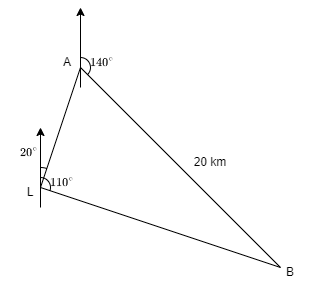
\includegraphics[scale=0.6]{f4finalq37.png}
    \end{figure} Find \begin{enumerate}
        \item the distance of $L$ from $B$,
        \item the bearing of $L$ from $B$.
    \end{enumerate}

    \hrulefill

        \hrulefill
            
        \hrulefill
        
        \hrulefill
        
        \hrulefill
        
        \hrulefill
        
        \hrulefill
        
        \hrulefill
        
        \hrulefill
        
        \hrulefill
        
        \hrulefill
        
        \hrulefill

        \hrulefill

        \hrulefill
            
        \hrulefill
        
        \hrulefill
        
        \hrulefill
        
        \hrulefill
        
        \hrulefill
        
        \hrulefill
        
        \hrulefill
        
        \hrulefill
        
        \hrulefill
        
        \hrulefill

        \hrulefill

        \hrulefill
            
        \hrulefill
        
        \hrulefill
        
        \hrulefill
        
        \hrulefill
        
        \hrulefill
        
        \hrulefill
        
        \hrulefill
        
        \hrulefill
        
        \hrulefill
        
        \hrulefill
            
        \hrulefill
        
        \hrulefill
        
        \hrulefill
        
        \hrulefill
        
        \hrulefill
        
        \hrulefill
        
        \hrulefill
        
        \hrulefill
        
        \hrulefill
        
        \hrulefill

    \pagebreak
    \item In the figure, $AB=4$, $AC=5$ and $BC=7$. Calculate $\angle A$ to the nearest degree.\begin{figure}[H]
        \centering
        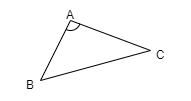
\includegraphics[scale=0.8]{f4finalq38.png}
    \end{figure}

    \hrulefill
        
        \hrulefill
            
        \hrulefill
        
        \hrulefill
        
        \hrulefill
            
        \hrulefill
        
        \hrulefill

    \item In the figure, find $AB$ and the area of $\triangle ABC$.\begin{figure}[H]
        \centering
        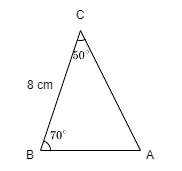
\includegraphics[scale=0.8]{f4finalq39.png}
    \end{figure}

    
        
        \hrulefill
            
        \hrulefill
        
        \hrulefill
        
        \hrulefill
        
        \hrulefill
        
        \hrulefill
        
        \hrulefill
        
        \hrulefill

    \pagebreak
    \item In the figure, $ABC$ is an equilateral triangle. $AB=2$. $D,E,F$ are points on $AB,BC,CA$ respectively such that $AD=BE=CF=x$.\begin{figure}[H]
        \centering
        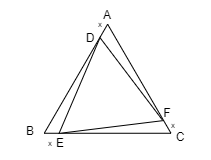
\includegraphics[scale=0.8]{f4finalq40.png}
    \end{figure}\begin{enumerate}
        \item By using the cosine formula or otherwise, express $DE^2$ in terms of $x$.
        \item Show that the area of $\triangle DEF=\dfrac{\sqrt{3}}{4}(3x^2-6x+4)$.
    \end{enumerate}
    \hrulefill
            
        \hrulefill
        
        \hrulefill
        
        \hrulefill
        
        \hrulefill
        
        \hrulefill
        
        \hrulefill
        
        \hrulefill
        
        \hrulefill
        
        \hrulefill
        
        \hrulefill
            
        \hrulefill
        
        \hrulefill
        
        \hrulefill
        
        \hrulefill
        
        \hrulefill
        
        \hrulefill
        
        \hrulefill
        
        \hrulefill
        
        \hrulefill
        
        \hrulefill

        \hrulefill
        
        \hrulefill
        
        \hrulefill
        
        \hrulefill
        
        \hrulefill
        
        \hrulefill
        
        \hrulefill
        
        \hrulefill
        
        \hrulefill
        
        \hrulefill
            
        \hrulefill
        
        \hrulefill
        
        \hrulefill
        
        \hrulefill
        
        \hrulefill
        
        \hrulefill
        
        \hrulefill
        
        \hrulefill
        
        \hrulefill
        
        \hrulefill
        
        \hrulefill
        
        \hrulefill
        
        \hrulefill
        
        \hrulefill
            
        \hrulefill
        
        \hrulefill
        
        \hrulefill
        
        \hrulefill

    \pagebreak
    \end{enumerate}
\end{document}